\section{Modelo de Despliegue}

\begin{figure}[h]

  \centering
  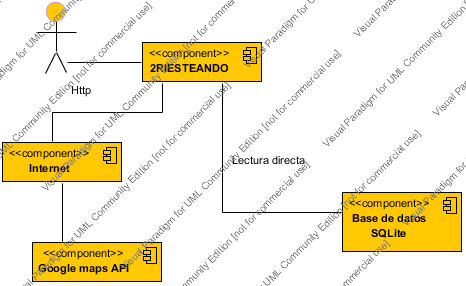
\includegraphics[width=14cm,height=6cm]{Imagenes/Despliegue/Arquitectonico.png}
  \caption{Diagrama de despliegue exterior}  
  \label{fig:arqui}
\end{figure}

El sistema interactuar\'a con una base de datos creada en SQLite 3, escribiendo directamente en ella, por otra parte realizar\'a una conex\'on
a internet a trav\'es del protocolo Http para obtener informaci\'on de la API de Google Maps versi\'on 2. Como
se muestra en la figura ~\ref{fig:arqui}.


\begin{figure}[h]

  \centering
  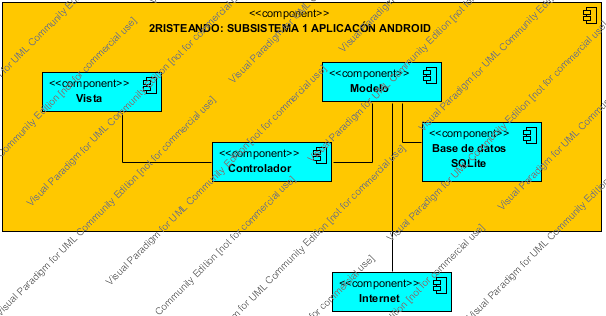
\includegraphics[width=18cm,height=6cm]{Imagenes/Despliegue/Subsistemas.png}
  \caption{Diagrama de despliegue interior}  
  \label{fig:subsistemas}
\end{figure}

El modelo de subsistemas est\'a representado en la figura ~\ref{fig:subsistemas}, el cual muestra el patr\'on de dise\~no
Modelo Vista Controlador. Donde la Vista ser\'a todo el conjunto de Activities que tendr\'a el sistema, el Controlador son
los eventos que controlar\'an la interacci\'on entre el Modelo y la Vista, finalmente, el Modelo tendra todo el funcionamiento
principal del sistema, como es calcular la ruta dependiendo el itinerario elegido o calcular un presupuesto seg\'un el n\'umero de personas
que asistan a dicha visita, interactuando con la base de datos que contiene el conjunto de informaci\'on de los lugares tur\'isticos
y la informaci\'on de los medios de transporte que pueden ser utilizados, as\'i como la interacc\'on con la API de Google Maps
para desplegar el mapa de la ciudad con los lugares seleccionados en el itinarario.